\documentclass{article}

% if you need to pass options to natbib, use, e.g.:
\PassOptionsToPackage{numbers, compress}{natbib}
% before loading preprint

\usepackage[preprint]{preprint}
\usepackage[authoryear]{natbib}


% to compile a camera-ready version, add the [final] option, e.g.:
% \usepackage[final]{preprint}


% to avoid loading the natbib package, add option nonatbib:
%\usepackage[nonatbib]{preprint}

\usepackage{bookmark}
\usepackage[utf8]{inputenc} % allow utf-8 input
\usepackage[T1]{fontenc}% use 8-bit T1 fonts
\usepackage{hyperref} % hyperlinks
\usepackage{url}% simple URL typesetting
\usepackage{booktabs} % professional-quality tables
\usepackage{amsfonts} % blackboard math symbols
\usepackage{nicefrac} % compact symbols for 1/2
\usepackage{microtype}% microtypography
\usepackage{xcolor} % colors
\usepackage{listings}
\usepackage{cite}
\usepackage{graphicx}
\usepackage{hyperref}
\usepackage{amsmath}
\renewcommand{\theequation}{}
\makeatletter
\@addtoreset{equation}{section}
\makeatother
\renewenvironment{equation}{\begin{equation*}}{\end{equation*}}
\usepackage{algpseudocode}
\usepackage{algorithm}
\usepackage{caption}
\usepackage{pdflscape}
\usepackage{tabularx}
\usepackage{multirow}
\usepackage{booktabs}
\usepackage{float}
\usepackage{longtable}

\lstset{
breaklines=true,
basicstyle=\ttfamily\small,
commentstyle=\color{green!40!black},
keywordstyle=\color{blue},
numberstyle=\tiny\color{gray},
numbers=none,
frame=single,
breaklines=true,
breakatwhitespace=true,
captionpos=b,
showstringspaces=false,
columns=fullflexible,
}

\hypersetup{
pdftitle={Scaling Speech LLM on Multi-Rate Discrete Speech Token Training},
pdfauthor={Husein Zolkepli},
pdfsubject={Audio and Speech Processing},
pdfkeywords={speech models, deep learning},
colorlinks=true,
linkcolor=blue,
citecolor=blue,
urlcolor=blue
}
\title{Multilingual-TTS: Scaling Discrete Speech Token Learning for Synthesis, Voice Cloning, and Expressive Control}
\author{
  Husein Zolkepli \\
  Scicom (MSC) Berhad, Malaysia \\
  \texttt{husein.zolkepli@scicom.com.my}
}


\begin{document}

\maketitle

\begin{abstract}
Most recent text-to-speech systems built on language models treat speech generation as a single task, leaving the joint scaling behavior of multilingual synthesis, voice cloning, and expressive control under a unified discrete token framework largely unexplored. In this work, we investigate whether a single autoregressive LLM can acquire all three capabilities from discrete audio tokens alone. We continue pretraining Qwen3 0.6B and 1.7B models across three training stages: a base multilingual TTS corpus covering 150+ languages with named speaker conditioning, a voice conversion corpus of paired utterances filtered by TitaNet speaker-embedding similarity, and an expressive TTS corpus where acoustic features (pitch, emotion, speaking rate, fluency, and noise characteristics) are extracted, binned, and converted into natural-language style descriptions by a large language model. All audio is tokenized by Neucodec at 50 tokens per second, allowing the model to treat speech generation as standard next-token prediction. On a 76-language evaluation benchmark, the 1.7B variant achieves a Character Error Rate of 0.2362 and a Mean Opinion Score of 3.2330, outperforming Dia TTS, Orpheus, and Fish Audio S2 Pro, while for voice cloning it reaches a speaker similarity of 0.5036 with a CER of 0.2656 across the same 76 languages. We additionally find that a hybrid Muon+AdamW optimizer strategy, applying Muon to 2D hidden layer weights and AdamW to embeddings and output heads, consistently outperforms AdamW alone under aggressive learning rate schedules. Because all inputs and outputs are discrete text-like tokens, the resulting models support streamable inference through standard LLM prefix caching. All models, datasets, and evaluation code are released at \url{https://github.com/Scicom-AI-Enterprise-Organization/Multilingual-TTS}.
\end{abstract}

\section{Introduction}

Large language models (LLMs) have rapidly expanded beyond text, with recent systems demonstrating impressive capabilities in vision, audio, and multimodal reasoning. In the speech domain, dominant approaches such as VoxTral (\citet{liu2025voxtral}) and Qwen2-Audio (\citet{chu2024qwen2audiotechnicalreport}) employ an encoder projection pipeline, a speech encoder first converts raw audio into continuous embeddings, which are then projected to match the LLM's embedding dimension before being inserted into the model in place of placeholder tokens. While this approach has enabled strong performance, especially in instruction-following and multimodal alignment tasks, it does not allow the LLM to natively operate over speech representations. The LLM sees only projected encoder outputs rather than actual audio tokens, restricting our ability to understand how LLMs learn from acoustic information and preventing direct scaling studies on speech tokenization.

Even when discrete audio tokens are used, an external encoder such as a neural codec remains necessary to generate token sequences from raw audio. However, discrete tokens fundamentally differ from projected encoder features, it can be incorporated into the LLM vocabulary as normal token IDs. By extending the vocabulary with a single discrete speech codebook, we allow the LLM to treat speech tokens on equal footing with text tokens. During continued pretraining, the LLM is exposed to paired sequences of discrete audio tokens and natural language transcripts, enabling it to learn a joint world model across the text and audio modalities. This approach requires no architectural modification, no learned modality-specific projection layer, and no injection of encoder features at inference time. Instead, the LLM directly models the statistical relationships between discrete acoustic sequences and textual output, similar to how it learns linguistic relationships during text-only pretraining.

Beyond architectural simplicity, this method offers practical benefits. Vocabulary extension is computationally inexpensive, the primary cost arises in the linear output head due to the increased vocabulary size. This cost scales linearly with token count and can be efficiently handled using optimized kernels such as the Liger cross-entropy kernel (\citet{hsu2025ligerkernelefficienttriton}). As a result, the overall training cost remains comparable to standard continued pretraining, even when incorporating tens of thousands of additional discrete tokens.

A central objective of this work is to study scaling behavior in discrete speech token learning, an area that remains largely unexplored. Prior research has not examined how LLMs learn from multi-rate discrete speech tokens or how model size interacts with token temporal resolution. To address this, we investigate two compact but capable model sizes, Qwen3 (\citet{yang2025qwen3technicalreport}) 0.6B and Qwen3 1.7B, and evaluate their ability to learn from multi-rate NeuCodec (\citet{julian2025finitescalarquantizationenables}) tokens at 6 Hz, 12.5 Hz, 25 Hz, and 50 Hz. These models provide a controlled setting in which scaling effects can be measured cleanly, enabling us to understand how discrete speech token learning behaves across both model capacity and temporal granularity.

Beyond scaling, encoder projection pipelines suffer from a significant deployment challenge, it breaks prefix caching, a core feature of modern inference engines such as vLLM (\citet{kwon2023efficientmemorymanagementlarge}) and SGLang (\citet{zheng2024sglangefficientexecutionstructured}). Because placeholder tokens use a single token ID and differ only in their post-embedding features, the LLM cannot reuse cached key-value states across inference steps. This forces full-sequence recomputation for every audio chunk, making streaming ASR infeasible. In contrast, discrete audio tokens are genuine vocabulary items, and each represents a unique token ID. As a result, prefix caching works exactly as it does in text-only LLMs. During streaming inference, the model needs only to append newly arriving audio tokens, while the cached context including previous audio remains intact. This allows the model to perform low-latency, incremental ASR with consistent contextual understanding and significantly reduced computation.

To evaluate this property, we additionally conduct continued finetuning on a chunked streaming dataset on top of the baseline models. This training exposes the LLM to segmented audio inputs with aligned transcripts and timestamps, enabling the model to process audio in short, incremental segments while maintaining continuity across chunks. With this training strategy, the LLM becomes capable of emitting transcriptions and timestamps progressively, achieving real-time responsiveness using standard LLM decoding workflows.

In summary, this work provides the first detailed study of LLMs trained directly on multi-rate discrete speech tokens, explicitly evaluating scaling behavior across 0.6B and 1.7B models. We demonstrate that discrete token continued pretraining offers a simple, architecture-preserving, and cache-compatible pathway to streamable speech recognition, revealing previously unexamined advantages of treating speech as an extension of the LLM's vocabulary rather than as an external modality handled by projection-based pipelines.

\section{Related Work}

Recent progress in speech-capable large language models has been driven largely by encoder-projection pipelines, where continuous speech representations are injected into an LLM through a learned projection layer. Systems such as VoxTral and Qwen2-Audio exemplify this dominant paradigm, a speech encoder produces high-dimensional continuous embeddings which are linearly projected into the LLM's embedding space and then consumed as pseudo-tokens. This strategy has enabled strong multimodal alignment and instruction-following performance, but it also imposes architectural complexity, prevents the model from learning native acoustic representations, and breaks prefix caching because embedding features cannot be represented as reusable token IDs.

A growing body of work instead explores representing speech as sequences of discrete audio tokens, enabling LLMs to process audio with vocabulary-level semantics. Early unified audio-text LMs, such as VioLA (\citep{wang2023violaunifiedcodeclanguage}) and LauraGPT (\citet{du2024lauragptlistenattendunderstand}), demonstrated that codec-based tokenization allows a transformer decoder to perform ASR, TTS, and AST using a single autoregressive model. These systems rely on neural codecs to convert raw audio into discrete units, which are then modeled generatively in the same manner as text. While these works highlight the potential of treating speech as tokens, they do not investigate how LLMs scale with discrete token rates, nor do they evaluate the effect of model size on learning acoustic-textual correspondences.

Other studies examine the limitations of existing quantizers, including the discrete representation inconsistency (DRI) problem, where identical speech segments may produce divergent token sequences, degrading the stability of downstream modeling (\citet{liu2024analyzingmitigatinginconsistencydiscrete}). Complementary analyses such as the Comparative Study of Discrete Speech Tokens for Semantic-Related Tasks with Large Language Models (\citet{wang2024comparativestudydiscretespeech}) show that continuous features often outperform discrete units in fine-grained semantic tasks, highlighting that discrete-token LMs remain under-explored and under-optimized relative to projection-based pipelines. Meanwhile, Review of Recent Advances in Discrete Speech Tokens (\citet{guo2025recentadvancesdiscretespeech}) provides a comprehensive taxonomy of codec-based and emergent-discrete representations, noting that scaling behavior in speech-LLMs remains an open question.

Several recent systems attempt to unify speech and text modeling within a single transformer without modality-specific modules. Language Models That Can Listen While Speaking (\citet{ma2024languagemodellistenspeaking}) investigate integrating both continuous and discrete speech sequences into a single autoregressive LM, demonstrating that audio tokens can coexist with textual tokens in a shared vocabulary. However, these approaches do not study multi-rate tokenization or how token temporal resolution affects LLM learning dynamics. Moreover, none of these prior works examine the interaction between LLM size, token frame rate, and training scale, leaving the scaling characteristics of discrete speech token learning essentially uncharted.

\section{Method}

This work studies whether large language models can acquire automatic speech recognition capabilities purely through continued pretraining on discrete audio tokens, without introducing architectural modifications, projection layers, or multimodal encoders inside the LLM. Our method is built around three core design principles, treating discrete speech tokens as first-class vocabulary items, scaling model size and token temporal resolution jointly to understand their interaction, and enabling efficient streaming ASR through compatibility with prefix caching. This section describes the full methodology, including tokenizer selection, vocabulary integration, multi-rate tokenization, continued pretraining, and streaming-oriented finetuning.

\subsection{Selecting the Audio Tokenizer}

The audio tokenizer plays a central role in our approach, as it defines the discrete interface through which the LLM perceives speech. Unlike encoder projection pipelines, where the encoder can compensate for deficiencies through its continuous representation, discrete-token-based models rely heavily on the tokenizer's ability to capture fine-grained acoustic and linguistic properties in a form that can be modeled autoregressively. Therefore, the tokenizer must satisfy three criteria, high perceptual quality across diverse languages, stable performance on languages unseen during the tokenizer's training, and the ability to produce tokens at multiple temporal resolutions without degrading intelligibility. We evaluate several candidates under these constraints, focusing primarily on NeuCodec (\citet{julian2025finitescalarquantizationenables}) and the improved XCodec (\citet{ye2024codecdoesmatterexploring}) variant recently proposed in Xcodec2-25TPS-24k (\citet{zolkepli2026improvingxcodec20multilingualspeech}).

The Xcodec2-25TPS-24k study benchmarks various neural audio tokenizers on the Common Voice (\citet{ardila2020commonvoicemassivelymultilingualspeech}) 17 test set across 116 languages and reports that NeuCodec achieves the highest performance measured by UTMoSv2 (\citet{baba2024t05voicemoschallenge2024}), an automatic MOS estimator widely used for perceptual audio evaluation. These results indicate that NeuCodec preserves the perceptual characteristics of speech better than competing codec-style models at similar token budgets. Importantly, UTMoSv2 evaluations correlate with intelligibility and overall acoustic fidelity, making NeuCodec an attractive choice for downstream ASR-oriented LLM training.

The same study introduces an enhanced XCodec2 model trained at 24 kHz and operating at 25 Hz. The author claim that this improved Xcodec2-25TPS-24k surpasses the baseline XCodec2 in both perceptual quality and linguistic consistency. However, their evaluation is limited to the Common Voice 17 test set, which contains languages that heavily overlap with those seen during tokenizer training. While such settings measure within-distribution performance, they do not assess the tokenizer's ability to generalize to new languages, a crucial requirement for large-scale multilingual ASR, especially when the downstream LLM is trained on more than 150 languages spanning diverse phonetic and phonological families.

To examine out-of-distribution robustness, we benchmark both NeuCodec and the improved XCodec2 model on Common Voice 22, which introduces a number of new languages absent from earlier versions of the dataset. Our evaluation follows the same automatic UTMoSv2 scoring pipeline as Xcodec2-25TPS-24k, ensuring a fair comparison. Surprisingly, the improved XCodec2 model not only fails to surpass NeuCodec on Common Voice 22 test set but also performs worse than the baseline XCodec2 on several newly introduced languages, including those with phonetic inventories markedly different from the languages used in the tokenizer's training set. This degradation suggests that the improved XCodec2 may be overfitted to the Common Voice 17 test set distribution or that its architectural modifications interact poorly with phonetic diversity outside its training domain.

In contrast, NeuCodec maintains consistent performance across both Common Voice 17 test set and Common Voice 22 test set. This stability is especially pronounced in languages with unique phonological structures (e.g., tone-heavy languages, click-consonant systems, or languages with complex vowel-length distinctions), where NeuCodec exhibits significantly more reliable reconstruction according to UTMoSv2 evaluations. The tokenizer's robustness indicates that it captures acoustic structure in a way that generalizes better to languages not explicitly present in the training data, a key requirement when training a single multilingual speech LLM.

Collectively, our findings show that NeuCodec is more robust, more generalizable, and more flexible than the improved XCodec2 model for large-scale multilingual discrete speech modeling. For these reasons, NeuCodec is selected as the audio tokenizer for all experiments in this work, providing discrete sequences at four temporal resolutions that serve as the sole speech input to our LLMs.

\subsection{Multi-Rate Discrete Tokenization}

A core objective of this work is to investigate how LLMs behave when trained on discrete speech tokens at different temporal resolutions. Prior speech LLM systems operate at a single fixed frame rate imposed by the architecture of their continuous audio encoders, leaving no room to study how temporal granularity affects downstream ASR performance or scaling behavior. In contrast, our approach exposes the LLM directly to four temporal resolutions, 50 Hz, 25 Hz, 12.5 Hz, and 6 Hz, all derived from a single NeuCodec codebook, enabling the first controlled study of multi-rate discrete token training.

To motivate the multi-rate design, we revisit the temporal characteristics of prominent encoder-based speech LLMs. VoxTral relies on the Whisper (\citet{radford2022robustspeechrecognitionlargescale}) large-v3 encoder, which converts audio into a 128-bin log-Mel spectrogram and applies a convolutional stem that halves the time resolution. The resulting features, after passing through a deep transformer stack, have a fixed 50 Hz frame rate determined entirely by Whisper's hop size and convolutional subsampling. Qwen2-Audio adopts a similar architecture but applies an additional pooling layer at the end of the encoder, yielding a fixed 25 Hz frame rate. The recently introduced Qwen3-Omni (\citet{xu2025qwen3omnitechnicalreport}) trains a new AuT encoder from scratch on 20 million hours of audio, and the outputs continuous embeddings at 12.5 Hz. While this offers computational advantages, the temporal rate is again determined by encoder pooling, and the LLM still does not operate directly on discrete tokens.

Across these systems, three constraints are consistent. First, the token rate is hard-coded by the encoder and cannot be varied without altering the model architecture. Second, the LLM only sees projected continuous vectors, not native token identities, preventing controlled analysis of what token rates the LLM actually prefers. Third, encoder projection pipelines prevent the LLM from performing prefix caching, which in turn blocks streamable ASR in modern inference engines.

NeuCodec differs fundamentally because it produces a sequence of discrete tokens at a natural resolution of 50 Hz. Since the output is a discrete sequence rather than a continuous feature stream, it becomes possible to derive alternative temporal resolutions without retraining or modifying the encoder. To create lower-rate versions, we reduce the sequence density by uniformly subsampling the discrete token sequence at fixed intervals. For example, selecting every second token yields a 25 Hz representation; selecting every fourth token yields a 12.5 Hz representation; and selecting every eighth token yields approximately 6 Hz. This uniform subsampling preserves token identity and requires no additional modeling assumptions. The resulting sequences differ only in temporal granularity, not in token semantics or codebook design.

NeuCodec is built on a HuBERT (\citet{hsu2021hubertselfsupervisedspeechrepresentation}) encoder, which performs bidirectional full-context attention processing each frame with both left-to-right and right-to-left context. As a result, the produced tokens already capture high-level semantic and phonetic structure of the audio, making them robust to temporal redundancy and allowing the LLM to operate directly on the full-resolution discrete sequence. Because HuBERT's masked-prediction training encourages each token to encode contextual meaning rather than purely local acoustic information, the discrete tokens remain informative even at higher frame rates (e.g., 25-50 Hz). Thus, unlike continuous-feature pipelines that must aggressively downsample to avoid excessive sequence lengths, NeuCodec tokens allow us to train the LLM without additional subsampling while preserving semantic integrity across time.

This strategy offers several advantages. Because all temporal resolutions originate from the same discrete vocabulary, the LLM can process them without architectural modification or the introduction of separate projection layers. Moreover, subsampling is deterministic and lossless at the token level, ensuring that multi-rate training requires no additional parameters or auxiliary modules. The differing rates spanning nearly an order of magnitude, also provide a natural axis for analyzing model behavior. For example, one can examine whether smaller models (0.6B) tend to prefer more compact, low-rate representations, whether larger models (1.7B) are able to exploit the fine-grained structure present in 50 Hz sequences, whether intermediate rates in the range of 12.5 to 25 Hz yield favorable trade-offs between sequence length, latency, and accuracy and whether scaling trends remain consistent across temporal granularities.

Taken together, multi-rate discrete tokenization enables a form of scaling analysis that has not been feasible in prior encoder-projection LLM architectures. Instead of being restricted by architectural design choices within an audio encoder, we can vary acoustic resolution independently of the LLM and treat temporal granularity as a controllable dimension of model scaling. This flexibility is unique to discrete speech tokenizers and constitutes a central pillar of the method introduced in this work.

\subsection{Building Large-Scale Multilingual Speech}

For continued pretraining, we construct a multilingual speech corpus exceeding 100{,}000 hours by aggregating a broad set of public, academic, community-curated, and synthetic datasets. Unlike the streaming-style finetuning corpus described later, the pretraining corpus uses a simple, uniform format: each sample is a pair consisting of an audio file and its plain-text transcription, as the objective is to expose the model to large-scale audio-text pairs rather than fine-grained segment structure.

\paragraph{Datasets with native transcriptions.}

The majority of datasets incorporated into our multilingual corpus provide native transcriptions that have been verified either by human annotators or semi-automatic quality-control pipelines. Leveraging these high-quality text–audio pairs, we compile a unified corpus that spans more than one hundred publicly available and community-contributed datasets, together covering over 150 languages and 59,378 hours of recorded speech. This breadth enables coverage across major language families, including Indo-Aryan, Dravidian, Afro-Asiatic, Sino-Tibetan, Austroasiatic, Austronesian, and European branches.

The corpus integrates a diverse range of speech styles and domains: expressive and emotional TTS corpora, multi-speaker conversational data, child and adult speech, audiobook narrations, accented and dialectal variations, and curated single-speaker studio datasets. This diversity is further enriched by synthetic corpora and pseudo-speaker augmentations, which expand the expressive space while maintaining consistent transcription quality.

All audio samples are standardized into discrete speech tokens using the 50 Hz neucodec tokenizer, resulting in 10.69 billion tokens used for pretraining our TTS models. A full catalog of all dataset sources is provided in the Malaysia-AI Multilingual-TTS repository.\footnote{\url{https://huggingface.co/datasets/malaysia-ai/Multilingual-TTS}}

\paragraph{Emilia-YODAS.}

We additionally incorporate the Emilia-YODAS (\citet{emilia}) dataset from Amphion (\citet{amphion}), post-processed by Scicom \footnote{ \url{https://huggingface.co/datasets/Scicom-intl/Emilia-YODAS-Voice-Conversion}}, which contributes substantial amounts of voice-converted multilingual speech: 5{,}558.53 hours of German, 13{,}493.57 hours of English, 6{,}954.43 hours of French, 1{,}120.36 hours of Japanese, 6{,}991.33 hours of Korean, and 326.01 hours of Chinese. These hours significantly expand the language coverage and speaker diversity available during pretraining.

\paragraph{Text-level post-filtering.}
\label{sec:text-label-post-filtering}

we apply rules to address transcription errors and hallucinations commonly observed in large ASR models. Specifically, we compute character ratio heuristic that flags segments with unusually high proportions of non-alphabetic characters, as well as a repetitiveness ratio that detects pathological word or subword repetition. Finally, we exclude segments containing hallucinated tokens or undesirable artifacts using the rejected-word list introduced in Granary (\citet{koluguri2025granaryspeechrecognitiontranslation}) especially for Emilia based dataset. Samples failing any of these linguistic or temporal criteria are removed.

\paragraph{Text-level post-processing.}
\label{sec:text-label-post-processing}

After text-level filtering, we apply an LLM-based normalization stage to restore punctuation and capitalization without modifying the lexical content of the transcript. This step uses the constrained prompting strategy introduced in Granary, which enforces strict edit rules allowing only punctuation and casing changes while prohibiting any insertion, deletion, or substitution of words. The model corrects missing or malformed punctuation, removes invalid symbols, and restricts all output to a fixed set of allowed marks, namely periods, commas, question marks, exclamation marks, semicolons, colons, and dashes. Sentence boundaries as well as interrogative and exclamatory forms are inferred from context, and capitalization is applied to sentence initials, proper nouns, and abbreviations. If the input already contains valid punctuation, it is left unchanged. This post-processing step improves readability and consistency while preserving the original ASR hypothesis.

We evaluate multiple instruction tuned LLMs for this normalization task, including Qwen/Qwen3-32B, Qwen/Qwen3-235B-A22B-Instruct-2507, and Qwen/Qwen2.5-72B-Instruct (\citet{qwen2025qwen25technicalreport}). Based on our internal benchmark measuring punctuation accuracy and constraint adherence, Qwen/Qwen2.5-72B-Instruct performs best and is therefore used in our pipeline.

\paragraph{Resulting dataset.}

After filtering and normalization, the combined corpus exceeds 100{,}000 hours of multilingual speech paired with plain-text transcriptions. This large-scale dataset forms the foundation of our continued pretraining experiments, enabling the model to learn robust acoustic and linguistic representations across a diverse range of languages, accents, and speaking styles.

\subsection{Building Whisper-Style Timestamped Segments}

After the large-scale continued pretraining stage, we perform a second finetuning phase designed to train the model on incremental, segment-level audio input. Instead of feeding each utterance as a single long sequence of discrete speech tokens, we adopt the Whisper-style segmentation format, where recordings are divided into short audio clips, each paired with a timestamped text snippet.

For each utterance, the dataset provides a list of timestamped text segments such as,

\begin{verbatim}
[
 "<|0.04|> Good morning everyone, and thank you for joining <|1.62|>",
 "<|2.20|> In this session we will discuss the progress <|4.38|>",
 "<|4.94|> and highlight several important findings from <|6.52|>",
 "<|7.10|> Our team has completed the first round <|8.24|>",
 "<|8.88|> and we are preparing the next set of experiments <|10.54|>",
 "<|11.12|> Before we move forward, let me summarize the <|12.98|>",
 "<|13.46|> model shows promising results in low-resource <|15.80|>"
]
\end{verbatim}

Each text entry contains explicit start and end timestamps corresponding to a specific time span in the original audio. The dataset also supplies the aligned audio clips as separate files:

\begin{verbatim}
[
 "segments/000123-0.mp3",
 "segments/000123-1.mp3",
 "segments/000123-2.mp3",
 "segments/000123-3.mp3",
 "segments/000123-4.mp3",
 "segments/000123-5.mp3",
 "segments/000123-6.mp3"
]
\end{verbatim}

Each audio file contains precisely the time region indicated by its paired text snippet. During finetuning, every audio clip is encoded into a sequence of discrete speech tokens using the NeuCodec tokenizer. We then construct training examples by interleaving audio and text segments in temporal order:

\begin{verbatim}
\end{verbatim}  

This structure teaches the model that each segment corresponds to a particular window of the utterance and that text must be generated locally for that segment. Because the input format alternates between short audio regions and their aligned transcripts, the model learns to perform incremental decoding: consume the audio for the current segment, produce the corresponding text, and then proceed to the next segment with full continuity of context.

Each training sample uses the same vocabulary as pretraining, consisting entirely of discrete speech tokens, timestamp markers embedded within the text, and standard text tokens. No monotonic attention mechanisms, projection layers, or alignment modules are added. The model learns the streaming behavior directly from the sequencing pattern.

By exposing the LLM to Whisper-style timestamped segments, this finetuning phase prepares the model for realistic streaming conditions, enabling accurate, chunk-by-chunk transcription without modifying the underlying architecture.

\subsubsection{Data Sources}
\label{sec:data-sources-streaming}

To construct a diverse and robust dataset suitable for both continued pretraining and streaming-style finetuning, we combine several multilingual and multi-domain speech corpora. The final dataset covers spontaneous conversational speech, parliamentary proceedings, scientific and technical discussions, and long-form podcast material. These sources were selected to ensure broad linguistic coverage, natural prosody, and a wide range of speaking styles.

\paragraph{Singaporean speech (IMDA).}
We include a substantial portion of the Singaporean speech corpus released by IMDA \footnote{ \url{https://huggingface.co/datasets/mesolitica/IMDA-STT}}. This dataset contains high-quality recordings across multiple accents of Singaporean English, with a mixture of prepared and spontaneous speech. It contributes valuable diversity in pronunciation patterns and speech rhythms commonly found in Southeast Asian English varieties.

\paragraph{Malaysian parliamentary proceedings.}
A large quantity of clean, long-form speech is obtained from recordings of the Malaysian Parliament. These sessions include formal debate, structured dialogue, and prepared statements, offering clear articulation and rich lexical variety. Parliamentary speech is particularly useful for training timestamped alignment models because speakers frequently produce well-defined pauses and phrase boundaries.

\paragraph{Scientific and technical content from YouTube.}
To expand the domain coverage, we scrape public educational content from YouTube using science-related keywords including \textit{computer science}, \textit{biology}, \textit{physics}, and \textit{general science}. These videos provide long-form monologues, lecture-style narration, and technical explanations. The academic vocabulary and structured discourse help the model handle specialized terminology and more complex syntactic constructions.

\paragraph{Malaysian podcasts.}
We additionally incorporate a collection of Malaysian podcasts covering a variety of genres such as interviews, casual discussions, and commentary. Podcast speech is generally conversational, less scripted, and acoustically varied, providing valuable examples of natural, spontaneous dialogue.

\subsubsection{Dataset Construction}

To support both large-scale continued pretraining and the subsequent streaming-style finetuning, we construct a high-quality multilingual speech-text dataset using a multi-stage pipeline. The objective of the pipeline is to generate reliable timestamped segment pairs from long-form audio while ensuring temporal consistency and transcription accuracy. The construction process consists of four major steps: (1) merging shorter audio clips into longer utterances, (2) computing word-level forced alignments, (3) segmentizing the aligned transcription based on silence, and (4) filtering low-quality or anomalous alignments.

\paragraph{Preparing raw audio and 30-second chunking.}
All audio sources in our corpus are raw and untranscribed. Before any alignment step, we split the recordings into segments of at most 30 seconds, following the maximum reliable input length supported by Whisper large-v3. Each long-form recording is therefore decomposed into a sequence of numbered 30-second chunks (e.g., \texttt{audio\_0001\_0.wav}, \texttt{audio\_0001\_1.wav}, \texttt{audio\_0001\_2.wav}, \ldots), preserving the original chronological ordering.

\paragraph{Pseudolabeling with Whisper large-v3.}
For every 30-second chunk, we generate an initial transcript using Whisper large-v3. These pseudolabels provide coarse segment-level timestamps and text that serve as input to the forced alignment stage. Because pseudolabels are computed independently for each chunk, all timestamps are initially local to the 30-second window.

\paragraph{Forced alignment.}
We then refine the Whisper pseudolabels using word-level forced alignment with Hugging Face CTC Models \citep{ashraf2024ctcforcedaligner}. The forced aligner provides start-end timestamps for each word within the chunk. Since each chunk originally corresponds to a fixed position in the long-form recording, we convert all timestamps into a global time coordinate by adding the appropriate offset computed from the chunk index. This produces a continuous, temporally coherent alignment across the entire utterance, even though alignment is performed per 30-second segment.

\paragraph{Silence-based segmentation.}
To prepare the aligned data for streaming-style finetuning, we identify phrase-level boundaries based on silence durations. Following common ASR segmentation practice, we start a new segment whenever the gap between consecutive aligned words exceeds 0.3 seconds. Each resulting segment forms a natural prosodic unit containing a contiguous sequence of words with minimal internal pauses. For every word within a segment, we create a Whisper-style timestamp token in the form:
\begin{verbatim}
<|start|> word <|end|>
\end{verbatim}
Concatenating these tokens yields a timestamp-annotated transcription aligned at word resolution.

\paragraph{Merging segments beyond 30 seconds.}
Although forced alignment and pseudolabeling operate on 30-second windows, the silence-based segmentation often produces segments that extend across the boundaries of adjacent chunks. To reconstruct longer, coherent segments, we merge any segment fragments whose aligned timestamps overlap or touch at chunk boundaries. This merging step ensures that the final dataset preserves the long-form continuity of the original recording, even though the pseudolabeling and alignment stages are limited to 30-second windows.

\paragraph{Quality filtering.}
Because both the transcription and word-level timestamps originate from model-generated outputs, Whisper large-v3 pseudolabels followed by CTC forced alignment, so we apply several layers of filtering to ensure that only high-quality, temporally consistent examples enter the training set. We first remove any aligned segments whose forced-alignment confidence scores fall below a dataset-specific threshold. In addition, we detect and discard timestamp anomalies indicative of alignment failures. A segment is rejected if the first word begins more than five seconds into the chunk, if any gap between consecutive words exceeds two seconds, or if any word duration is longer than one second.

Beyond alignment-based filtering, we also apply the text-level post-filtering procedure described in Section~\ref{sec:text-label-post-filtering}. Together, these filtering steps ensure that the final dataset contains only reliable Whisper-style timestamped segments with consistent temporal structure and stable lexical content.

\paragraph{Motivation for filtering.}
Both the transcription and the word-level timestamps in our pipeline are produced entirely by models: Whisper large-v3 generates pseudolabels for each 30-second chunk, and the subsequent word-level timings come from the CTC-based forced aligner. Because neither source is ground truth, errors can accumulate in regions with noise, overlapping speech, accented pronunciations, or low-quality recordings. In practice, the forced aligner occasionally assigns incorrect boundaries, overly long word durations, or large gaps between consecutive words. To mitigate these issues, we apply strict filtering based on the confidence scores returned by the forced aligner, removing any segments whose alignment confidence falls below a threshold. We additionally discard segments exhibiting timestamp anomalies to ensure that only stable, high-quality Whisper-style timestamped segments are included in the final dataset.

\paragraph{Resulting dataset.}
After all transformation and filtering steps, the post-training corpus contains roughly 20{,}000 hours of clean, timestamp-aligned speech. Each example consists of a list of short, temporally coherent segments, where every segment includes (1) an audio clip extracted according to the forced-alignment timestamps, and (2) its corresponding Whisper-style timestamped transcription. This dataset serves as the foundation for our streaming-oriented finetuning stage and provides high-quality chunk-level audio--text pairs suitable for incremental ASR modeling.

Together, these post-training sources form a diverse long-form speech dataset with high temporal precision after alignment and filtering, enabling the model to learn stable speech-to-text behavior under streaming and segment-level decoding conditions.

\section{Experiments}

\paragraph{FlashAttention-3 with bfloat16 activations.}
All experiments are trained using FlashAttention-3 \citep{shah2024flashattention3fastaccurateattention} with \texttt{bfloat16} activations. FlashAttention-3 provides substantial throughput gains for long-context transformer training, and in our setup we observe approximately a $2\times$ throughput compared to a FlashAttention-2 baseline \citep{dao2023flashattention2fasterattentionbetter}. This improvement is consistent with the results reported in the FlashAttention-3 paper. The increased efficiency is particularly important in our setting, where the use of very large vocabularies derived from discrete speech tokenization makes attention computation the dominant training cost.

\paragraph{Dynamic multi-packing for a 10{,}240-token context window.}
Because our training sequences consist of highly variable lengths ranging from short streaming segments to long-form audio transcripts naively batching samples wastes significant context capacity due to padding. To fully utilize the available 10{,}240-token context length, we employ a \emph{dynamic multi-packing} strategy inspired by bin-packing algorithms, maximizing token density and reducing padding to nearly zero.

This approach yields several benefits. First, it enables a much higher effective batch size, since many more sequences can be packed into a single forward pass compared to naive batching. Second, GPU utilization improves substantially: most of the computation and memory footprint is spent on ``real'' tokens rather than on padding introduced by uneven sequence lengths. Third, dynamic multi-packing leads to more stable optimization dynamics. When batching naively, short sequences dominate the batch and introduce large variance in token-level gradients; by contrast, packing sequences of mixed lengths into near-maximal context windows produces smoother gradients and more consistent training behavior.

\paragraph{Mixed-precision configuration: FP32 weights vs.\ BF16 weights.}

Models trained with NeuCodec's 65{,}536-token vocabulary are particularly sensitive to numerical precision in the embedding tables and output projection layer. To quantify this effect, we perform a controlled ablation on Qwen3-0.6B using a single H100 GPU. We compare two precision configurations over 1{,}000 training steps: (i) both weights and activations in \texttt{bfloat16}, and (ii) FP32 weights with \texttt{bfloat16} activations. All other variables---optimizer, learning-rate schedule, global seed, and dataloader configuration---are held constant to isolate the impact of weight precision.

Across all measurements, the FP32-weight configuration consistently achieves better optimization stability and lower loss. After 1{,}000 steps, FP32 weights reach a loss of 9.18, compared to 9.81 for the BF16-only configuration:

\begin{center}
\begin{tabular}{lcc}
\toprule
\textbf{Precision Setting} & \textbf{Loss (1k steps)} $\downarrow$ \\
\midrule
BF16 weights / BF16 activations & 9.81 \\
FP32 weights / BF16 activations & \textbf{9.18} \\
\bottomrule
\end{tabular}
\end{center}

In addition to step-based comparison, we also evaluate convergence under a fixed wall-clock budget. At exactly 24 minutes of training time, the FP32-weight run achieves a lower loss (9.1) than the BF16-only run (9.7), demonstrating that improved numerical stability offsets the additional computational overhead. A figure for the wall-clock convergence plot is shown below,

\begin{figure}[h]
    \centering
    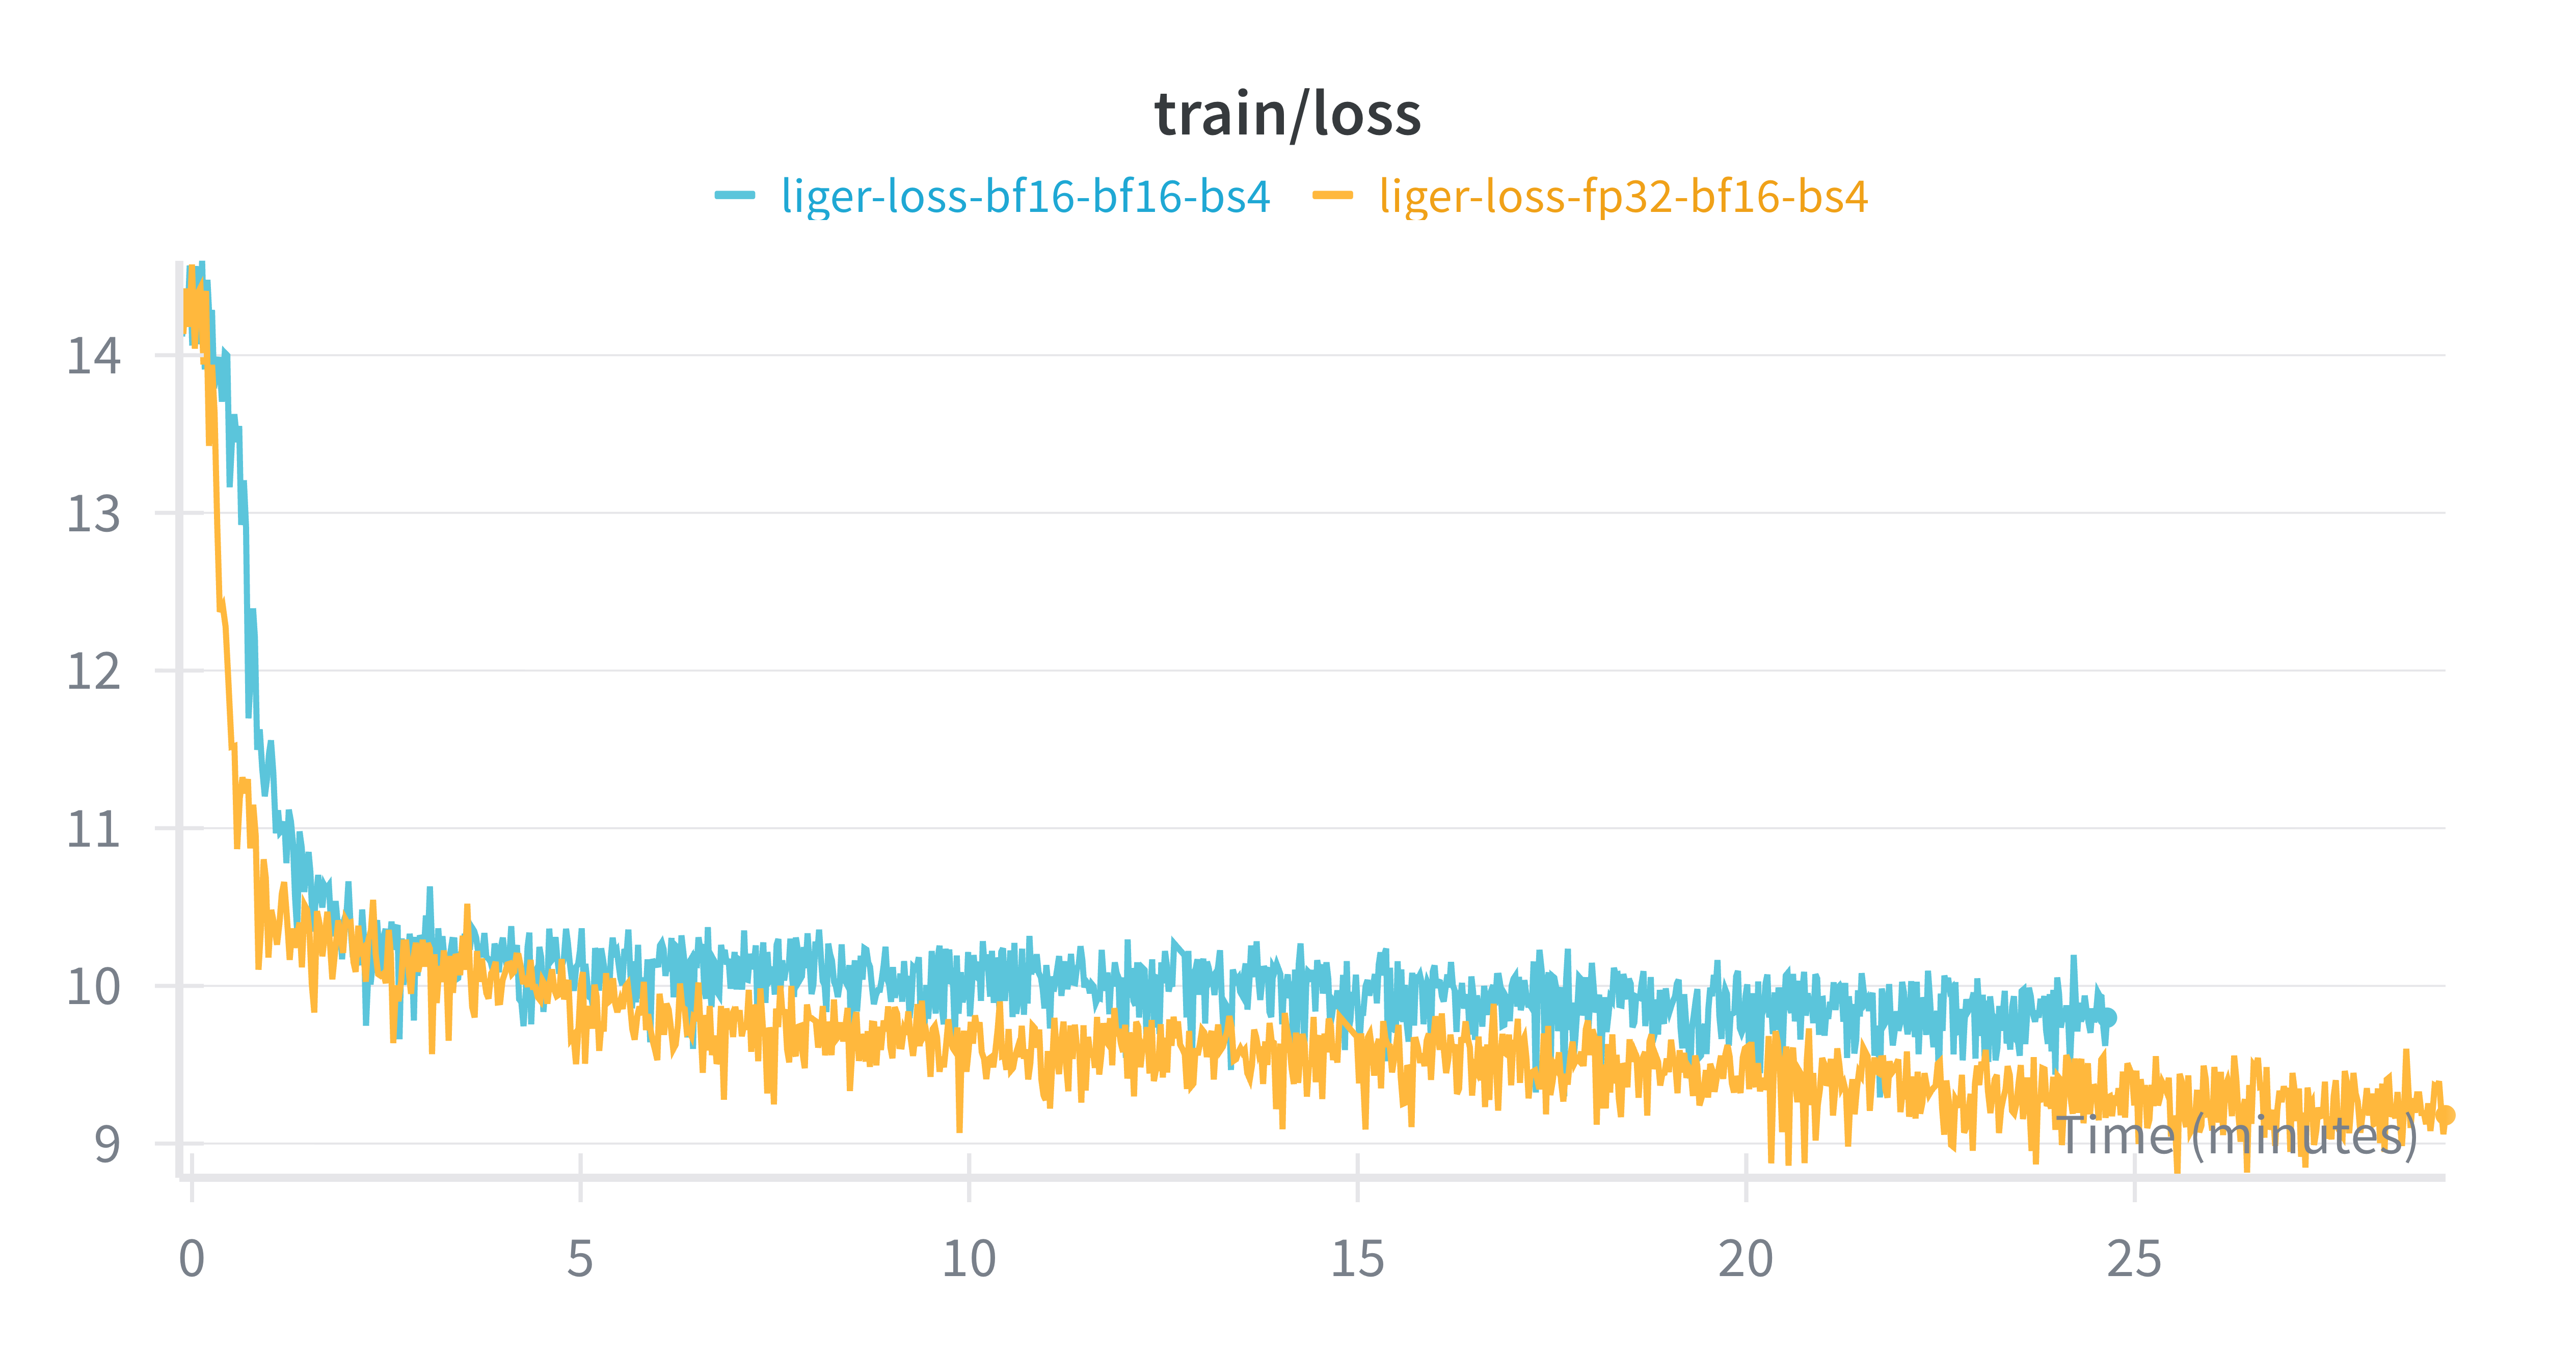
\includegraphics[width=0.85\linewidth]{wb-wallclock.png}
    \caption{Loss vs.\ wall-clock time for FP32 vs.\ BF16 weight precision.}
    \label{fig:loss_wallclock}
\end{figure}

We also measure Model FLOP Utilization (MFU). As expected, FP32 weights incur a lower MFU (47\%) compared to BF16 weights (56\%), indicating a reduction in hardware efficiency:

\begin{figure}[h]
    \centering
    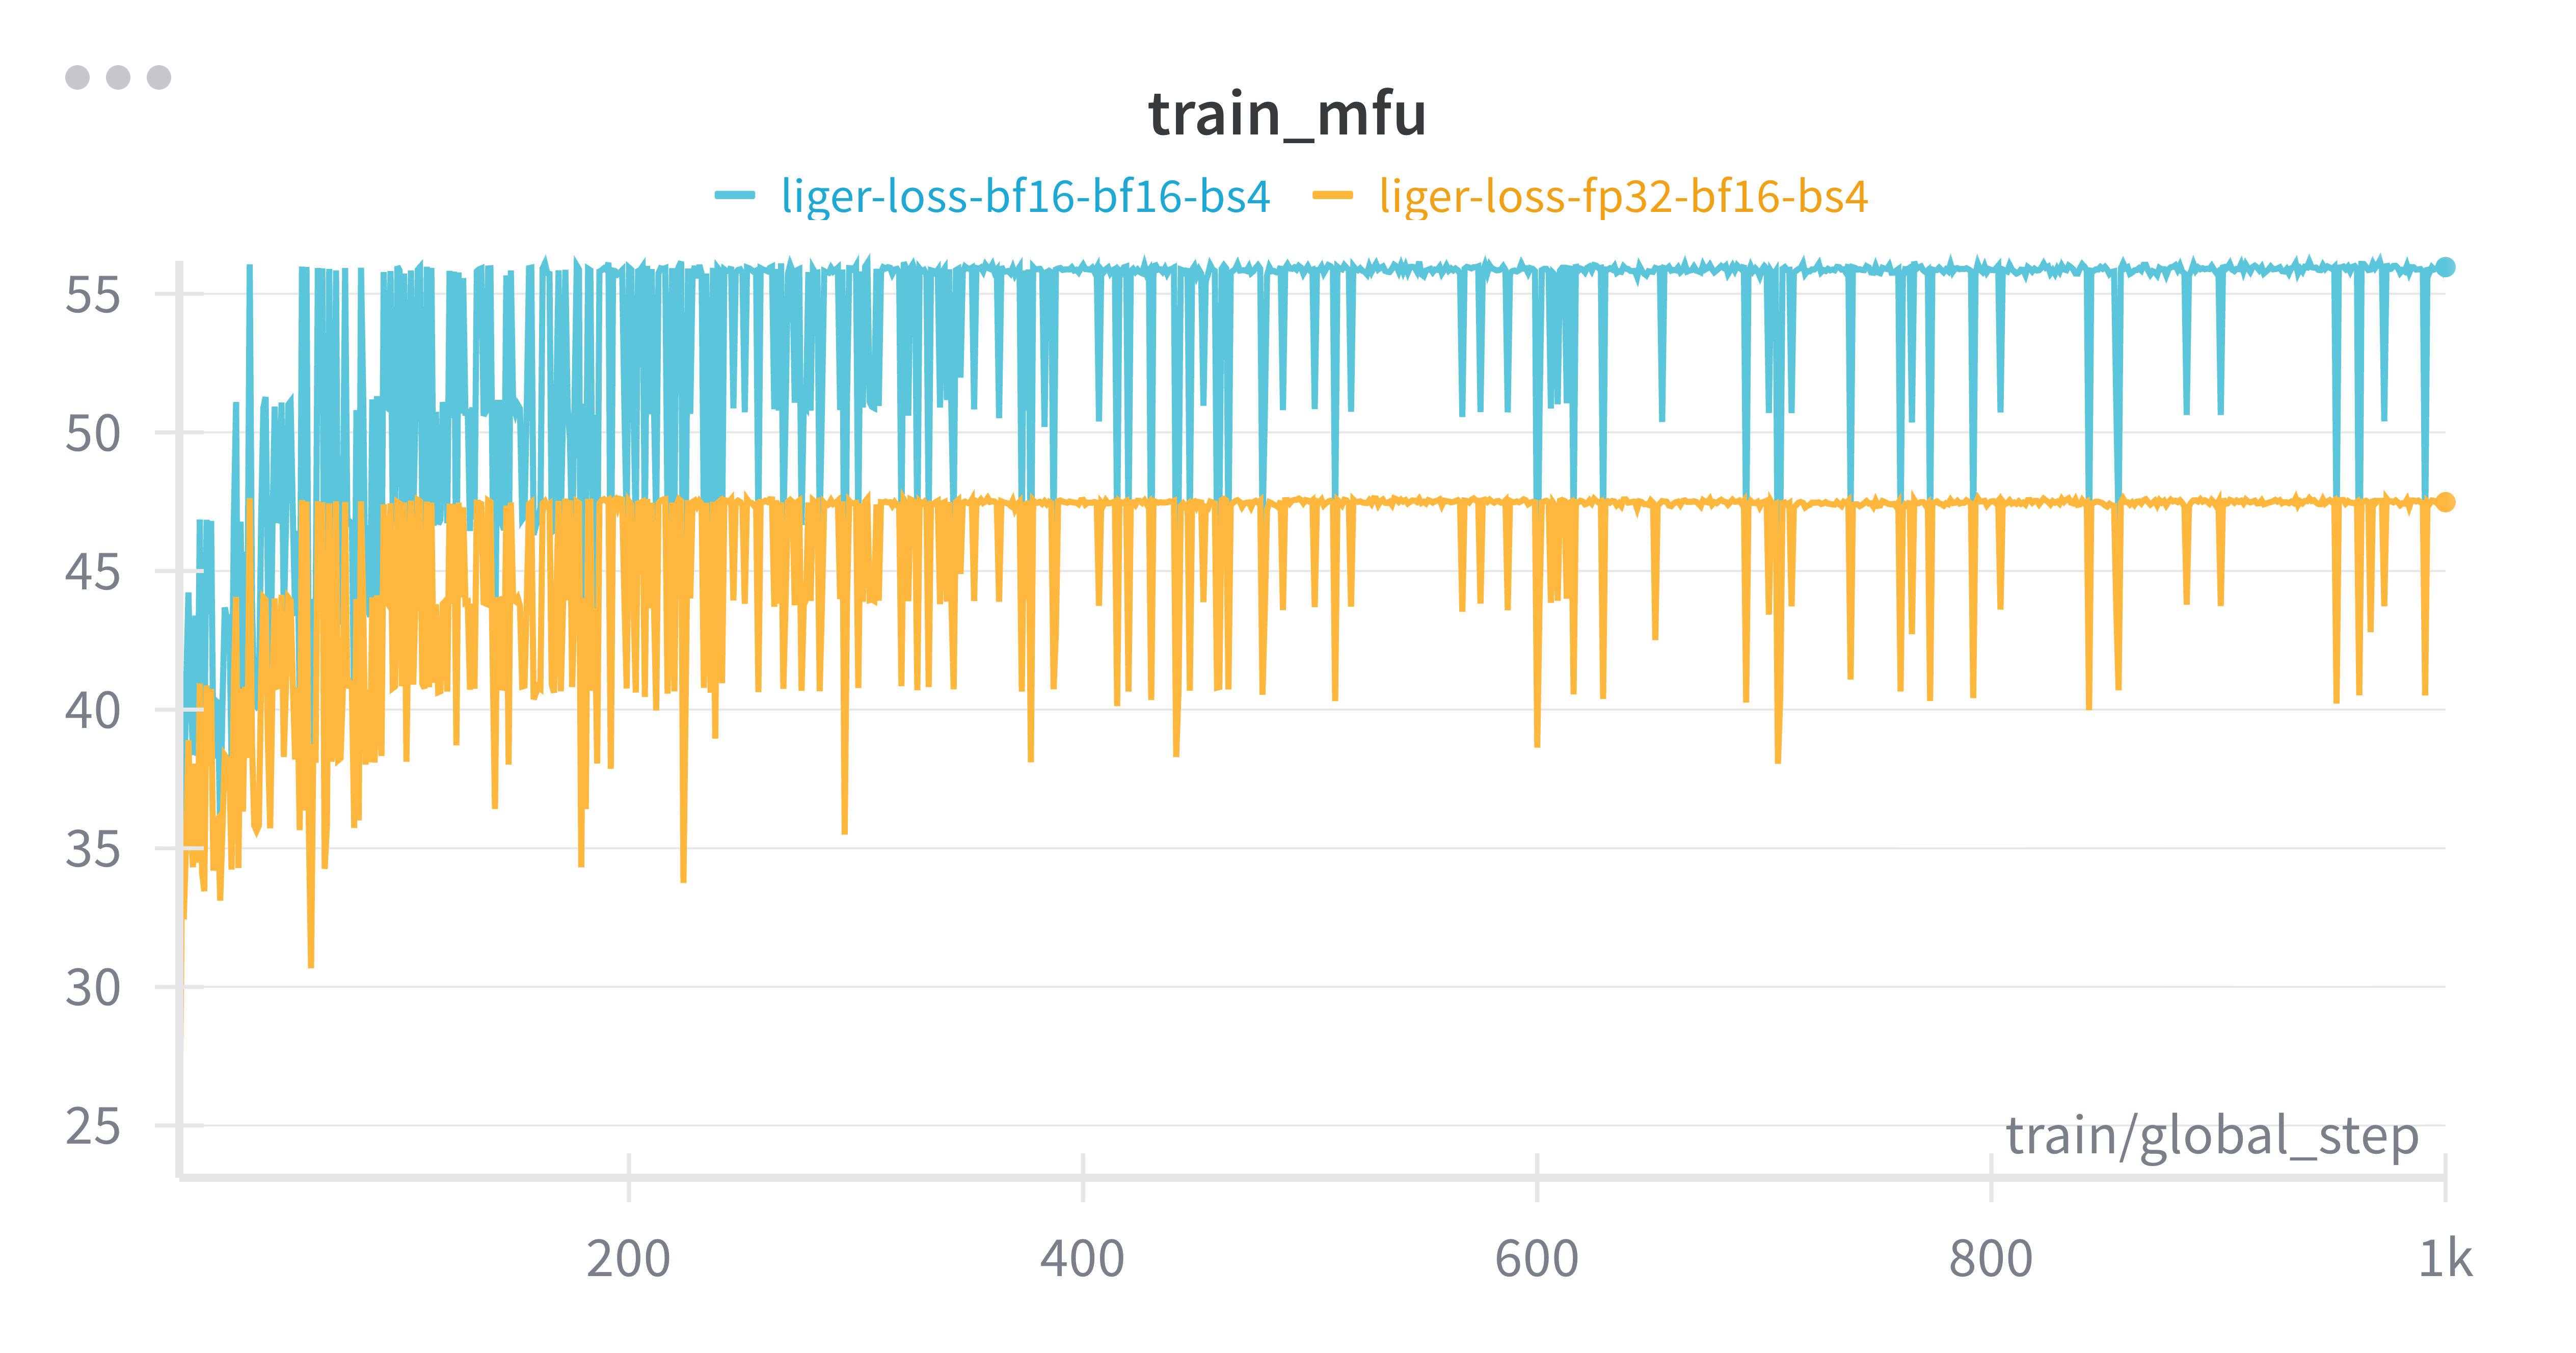
\includegraphics[width=0.85\linewidth]{wb-mfu.png}
    \caption{MFU achieved under each precision configuration.}
    \label{fig:loss_mfu}
\end{figure}

Despite this lower MFU and correspondingly longer time-to-step, the FP32-weight configuration still outperforms BF16 at equal wall-clock time. This suggests that, for large discrete-code vocabularies such as NeuCodec (65k tokens), the additional numerical precision in the embedding and output layers meaningfully improves training dynamics. In practice, the improved convergence rate more than compensates for the reduced throughput, leading to better model quality under identical time budgets.

\paragraph{Fused cross-entropy: Liger loss vs.\ Apple CCE.}

We also compare two fused cross-entropy implementations commonly used for large-vocabulary language modeling: the Liger fused linear cross-entropy kernel and the Apple fused CCE implementation (\citet{wijmans2025cutlosseslargevocabularylanguage}). For Apple CCE, we use the \texttt{cce\_kahan\_full\_c} reduction mode, which provides improved numerical compensation for large logits and vocabulary sizes. Using the same Qwen3-0.6B setup as in the previous section (FP32 weights + BF16 activations), we perform a 1{,}000-step ablation. Liger loss achieves the lowest training loss:

\begin{center}
\begin{tabular}{lcc}
\toprule
\textbf{Loss Function} & \textbf{Loss (1k steps)} $\downarrow$ \\
\midrule
Apple fused CCE (\texttt{cce\_kahan\_full\_c}) & 9.31 \\
Liger fused linear cross-entropy & \textbf{9.17} \\
\bottomrule
\end{tabular}
\end{center}

To further analyze convergence under equal wall-clock time rather than equal step count, we compare both loss functions at exactly 27 minutes of training. Liger again achieves a lower loss (9.197) relative to Apple CCE (9.265), suggesting that its improved numerical formulations translate into faster real-time convergence:

\begin{figure}[h]
    \centering
    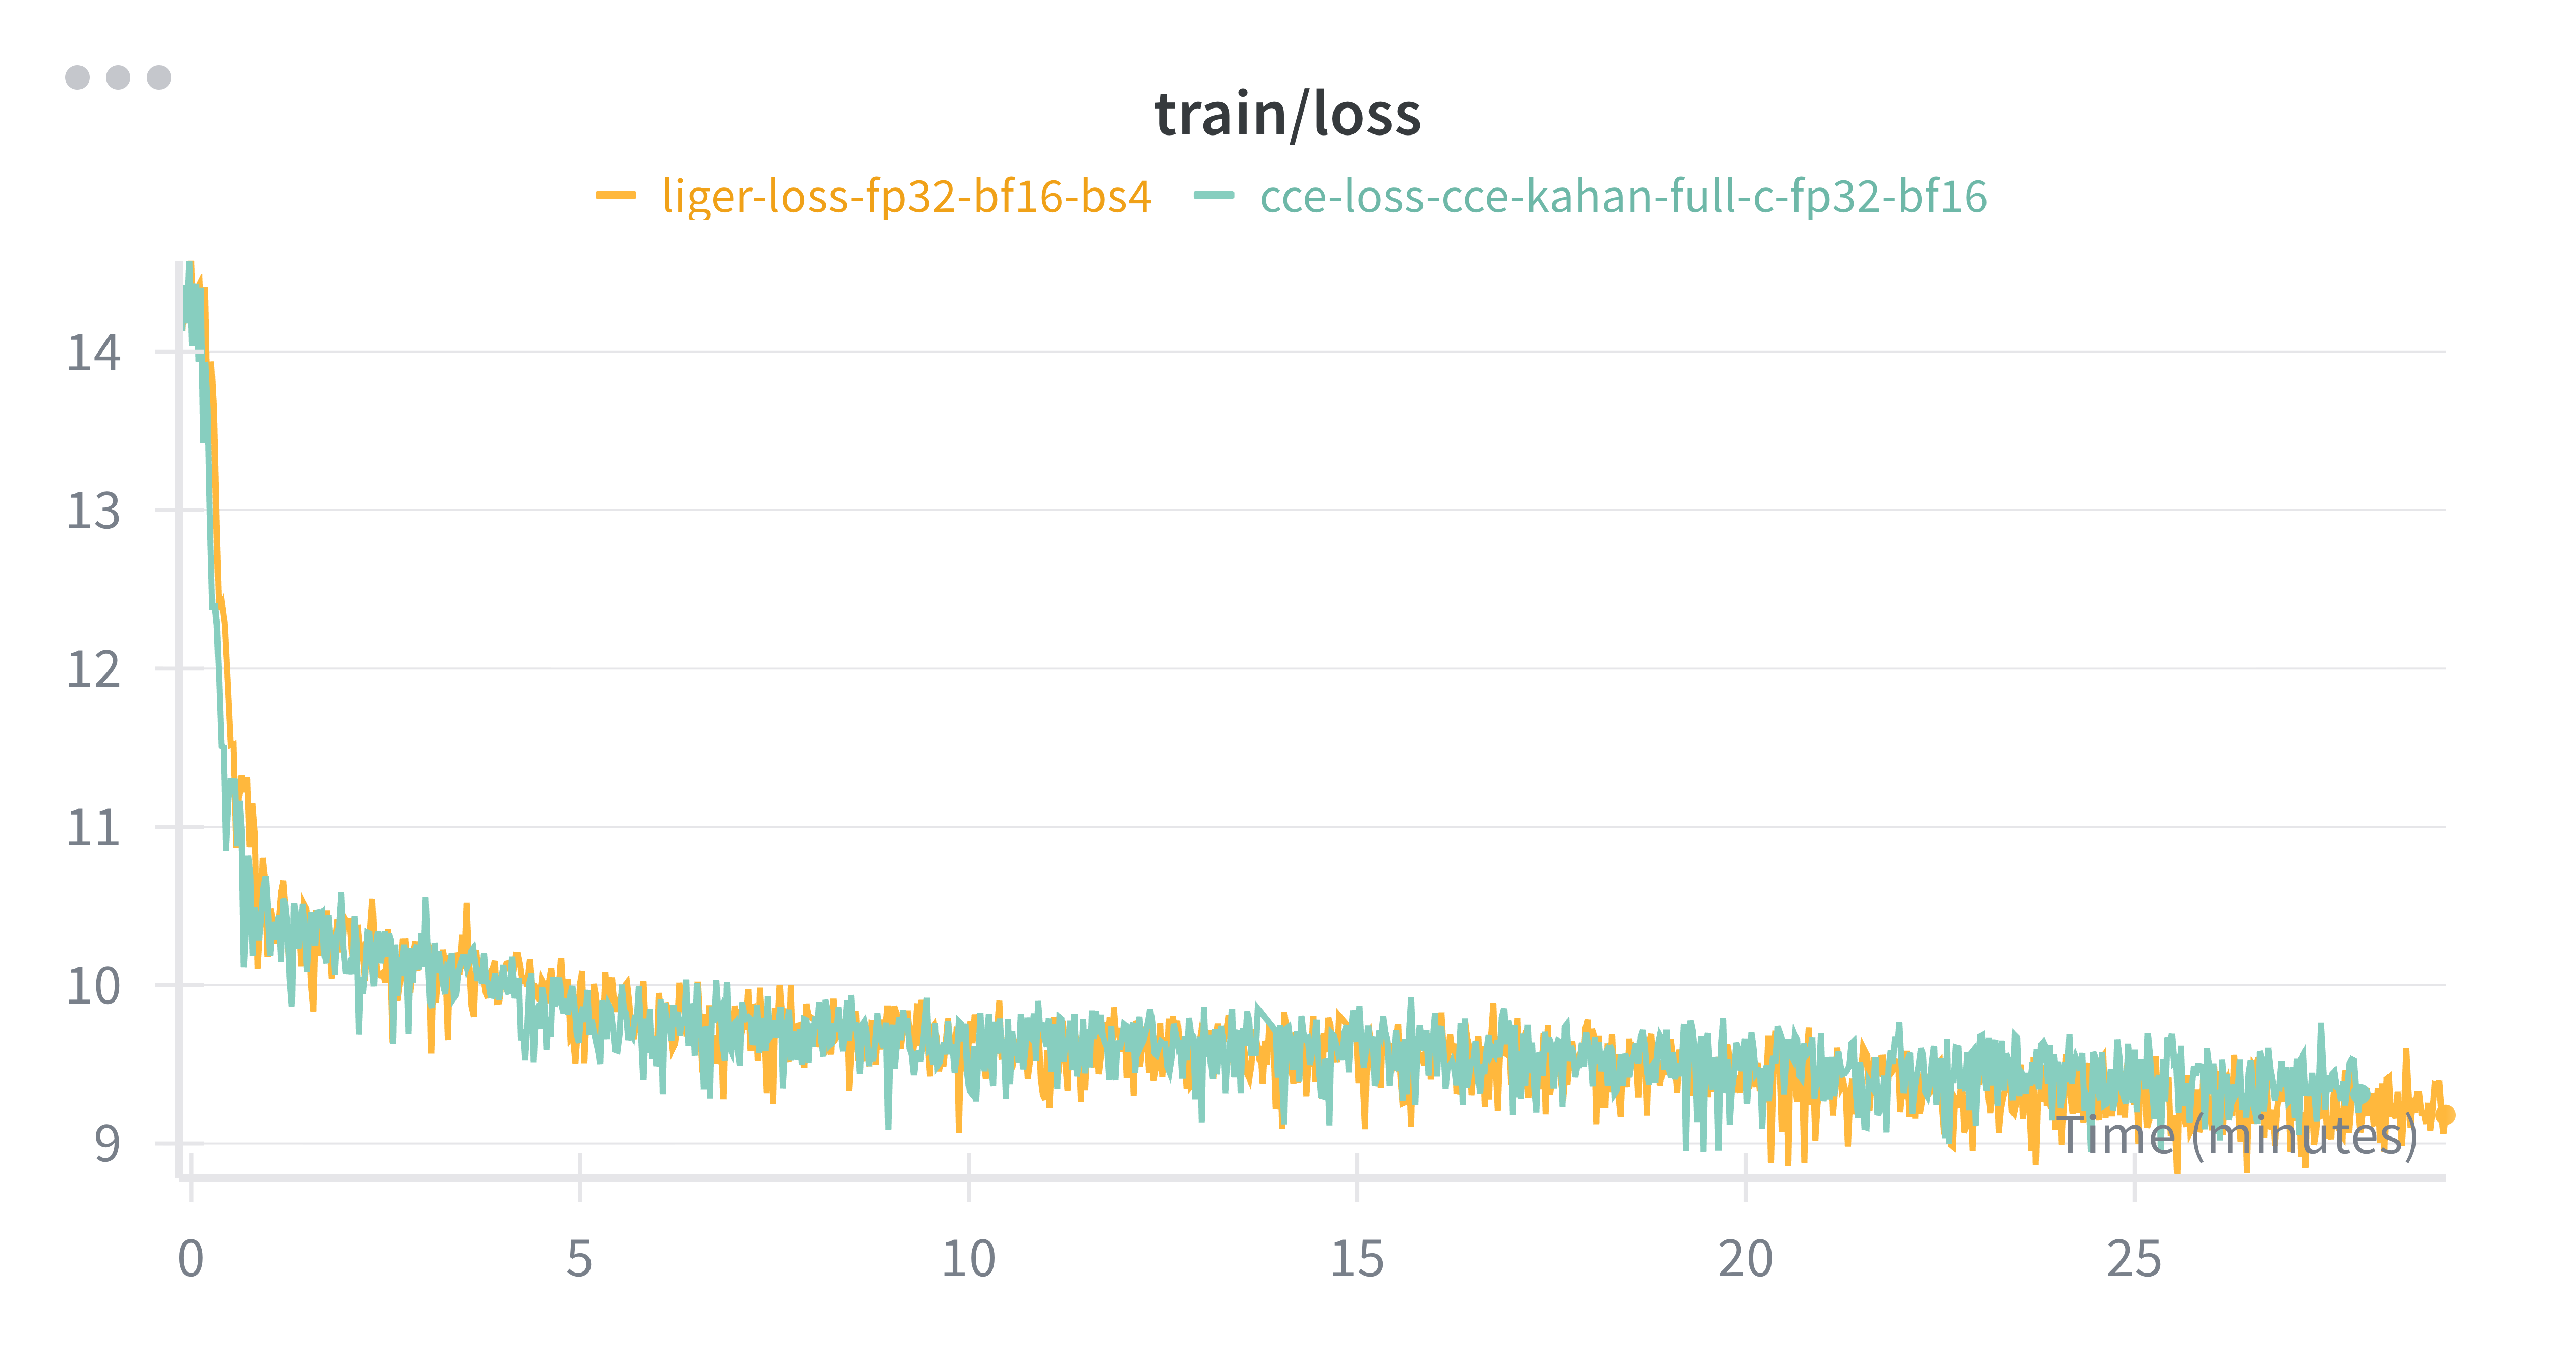
\includegraphics[width=0.85\linewidth]{wb-loss-liger.png}
    \caption{Loss vs.\ wall-clock time for Liger vs.\ Apple fused CCE.}
    \label{fig:loss_mfu}
\end{figure}

We also measure MFU and observe that both implementations achieve essentially identical hardware utilization throughout training, indicating that the performance difference arises from numerical properties of the loss computation rather than from kernel-level throughput characteristics:

\begin{figure}[h]
    \centering
    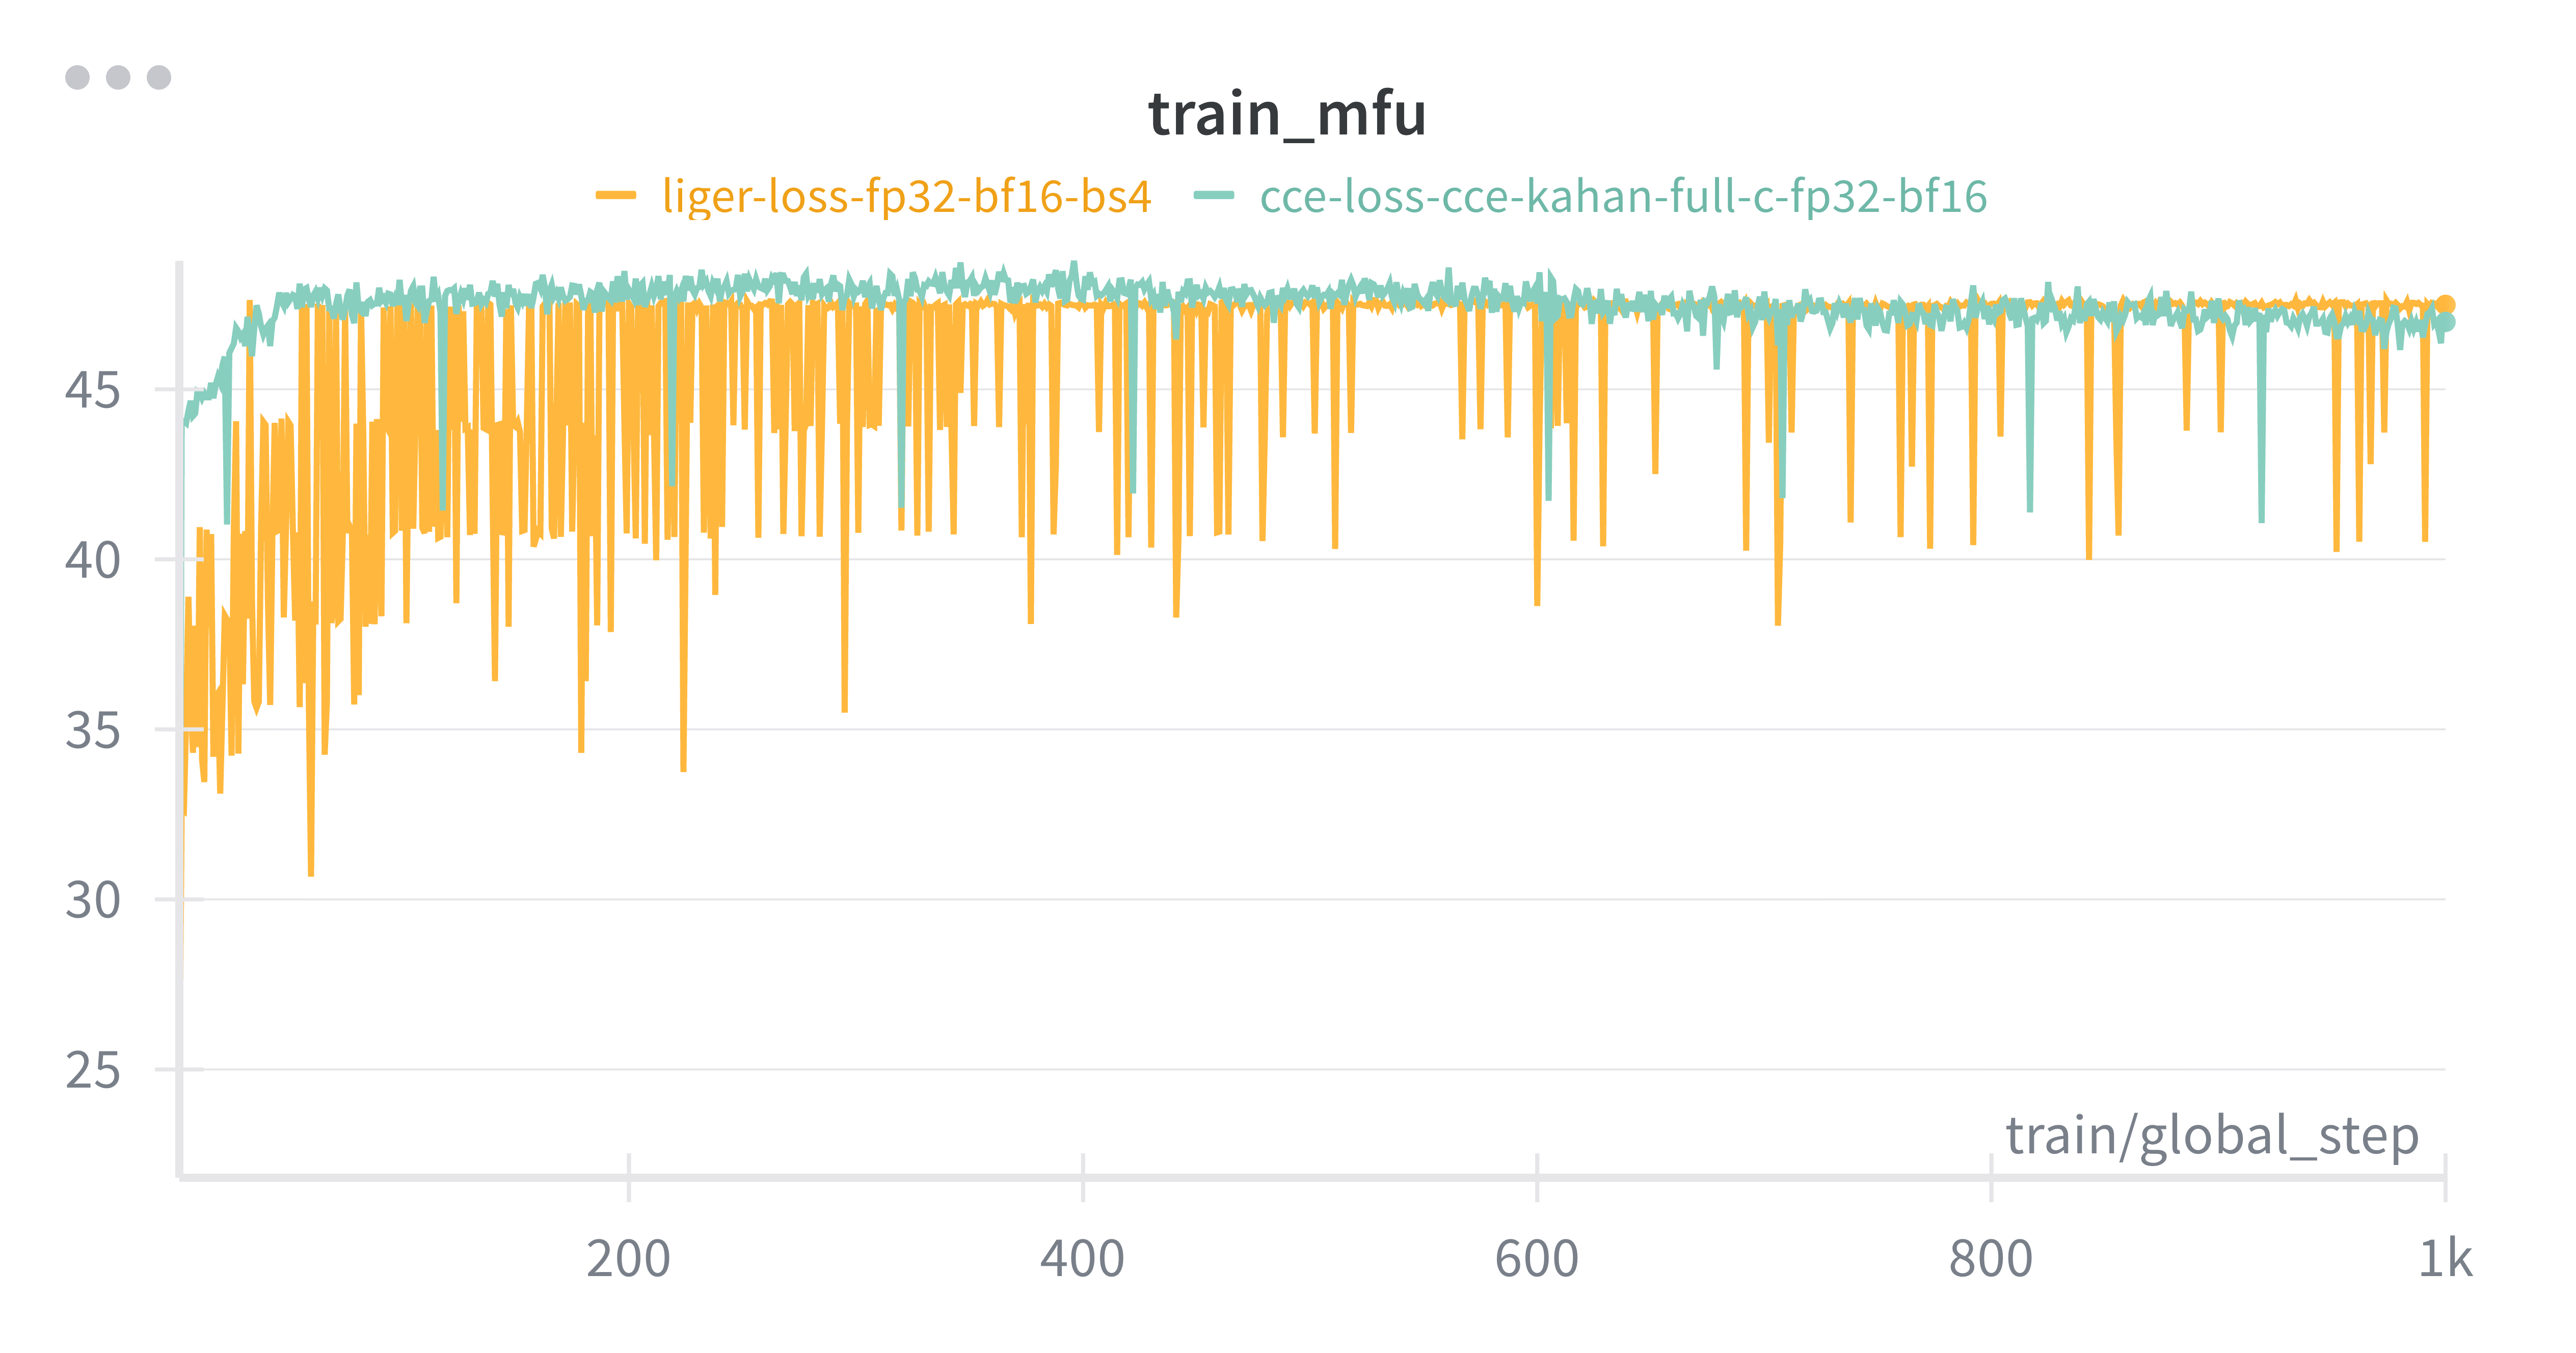
\includegraphics[width=0.85\linewidth]{wb-mfu-liger.png}
    \caption{MFU for Liger fused linear CE and Apple fused CCE.}
    \label{fig:loss_mfu}
\end{figure}

Taken together, these results suggest that Liger's fused linear cross-entropy kernel provides more stable optimization behavior for large-vocabulary setups such as NeuCodec (65k tokens), yielding better convergence both per training step and per unit of wall-clock time. The small ablation experiments available at Scicom-AI-Enterprise-Organization/small-ablation repository. \footnote{ \url{https://github.com/Scicom-AI-Enterprise-Organization/small-ablation/tree/main/liger-vs-cce}}

\subsection{Continue Pretraining on Large-Scale Multilingual Speech}

To analyze how model size and token rate affect convergence, we track training loss across all 
continued-pretraining runs. For each model size (0.6B and 1.7B), we train five variants: 
one for each NeuCodec temporal resolution (6~Hz, 12.5~Hz, 25~Hz, and 50~Hz), and one 
\emph{merged-rate} model trained on a mixture of all four token rates. This yields a total of 
ten pretraining curves.

Insert graph and describe.

\subsection{Post-Training on Whisper-Style Timestamped Segments}

For the timestamp-based post-training stage, we finetune only the merged-rate continued-pretraining 
checkpoints. This choice reflects a practical deployment scenario in which a single model must 
handle arbitrary token rates and streaming inputs. All post-training runs therefore begin from 
the merged-rate checkpoints of the 0.6B and 1.7B models and are trained exclusively on 
Whisper-style timestamped segments.

During post-training, both model sizes rapidly adapt to the timestamp supervision format. The 1.7B merged-rate model exhibits faster convergence and lower alignment loss, while the 0.6B model converges more slowly but remains stable throughout training. Notably, after only 1{,}000 post-training steps the models are already able to generate reasonably accurate token-level boundaries with timestamps: we observe clear `<|start|>` and `<|end|>` behavior in the decoded outputs. Because the post-training dataset contains fine-grained segment boundaries, this stage helps the model learn timestamp-aware behavior needed for stable streaming ASR.

Insert graph and describe.

\section{Evaluation}

We evaluate all models using character error rate (CER) and word error rate (WER) computed with the \texttt{jiwer} library \footnote{ \url{https://github.com/jitsi/jiwer}}. To ensure stable metric behavior across multilingual test sets, we apply two normalization procedures prior to scoring.

First, following common practice in multilingual ASR evaluation, we convert reference and hypothesis text to lowercase and remove punctuation. This reduces superficial discrepancies between languages with different orthographic conventions and improves comparability with other multilingual ASR systems that adopt similar normalization pipelines.

Second, we cap both CER and WER at a maximum value of~1.0. This clipping is necessary because several widely used ASR baselines most notably Whisper large-v3 and Whisper large-turbo-v3 occasionally produce repetition transcripts on certain multilingual utterances. These failure cases can result in unbounded error values that distort aggregated metrics. Applying a ceiling of~1.0 ensures that extreme outliers do not overwhelm the average error rates while still preserving the relative ordering between systems.

All scores reported in the following sections adopt these normalization and clipping rules.

\subsection{Multilingual Evaluation Dataset}

For multilingual ASR evaluation, we use the Common Voice 22 test set, which covers 160 languages. To ensure consistency across languages and to remove extremely short or long utterances that can distort CER and WER, we apply a duration-based filtering step: only audio samples longer than one second and shorter than twenty seconds are retained.

After applying the duration filter, we construct a balanced evaluation subset by selecting at most 1{,}000 samples per language. For each language, the filtered utterances are sorted by duration, and the first 1{,}000 examples are chosen. This procedure guarantees that every language contributes a comparable number of evaluation samples while preserving diversity in speaking rate and acoustic conditions. The complete evaluation set is publicly available at Scicom-intl/filtered-common-voice-22-test \footnote{ \url{https://huggingface.co/datasets/Scicom-intl/filtered-common-voice-22-test}}.

\subsection{Results Across Token Rates}

\subsection{Streaming Evaluation Dataset}

To evaluate streaming performance, we construct a timestamp-aligned evaluation set derived from 
four multilingual and multi-domain speech sources: (i) Singaporean speech from IMDA, 
(ii) Malaysian parliamentary proceedings, (iii) scientific and technical educational material 
from YouTube, and (iv) Malaysian podcasts, same source from Section~\ref{sec:data-sources-streaming}. From each source we extract exactly 10 hours of 
speech, yielding a 40-hour, multi-accent, multi-domain streaming benchmark.

\paragraph{Evaluation for our models.}
Our Qwen3-based models (0.6B and 1.7B) are evaluated on the full 40-hour multilingual 
streaming benchmark using incremental chunk-based decoding. At each timestep, a new audio 
segment is appended and processed under prefix caching. For every decoding step, we compute 
three metrics: (1) character error rate (CER), (2) word error rate (WER), and 
(3) timestamp distance. The timestamp distance measures the absolute deviation between the 
predicted <|start|> and <|end|> boundaries and the corresponding ground-truth timestamps 
provided by forced alignment. This metric captures the temporal accuracy of the streaming 
decoder and reflects how well the model maintains alignment across segment boundaries. All 
metrics incorporate the normalization, lowercasing, and 1.0-error capping described earlier.

\paragraph{Evaluation for external baseline models.}
For external speech-capable LLMs and ASR baselines such as Voxtral, Gemma-3N (\citet{gemmateam2025gemma3technicalreport}), Granite Speech (\citet{saon2025granitespeechopensourcespeechawarellms}), 
Phi-4 multimodal variants (\citet{microsoft2025phi4minitechnicalreportcompact}), Qwen2-Audio, Qwen2.5-Omni (\citet{xu2025qwen25omnitechnicalreport}), UltraVox \footnote{ \url{https://huggingface.co/fixie-ai/ultravox-v0_6-llama-3_3-70b}}, and Whisper-based 
models, and we restrict evaluation to the English portion of our streaming benchmark, namely 
Singaporean English (IMDA) and the YouTube scientific technical subset. Many of these models 
do not support timestamp prediction, so we evaluate them using only CER and WER, applying the 
same normalization and 1.0-error capping described earlier.

\subsection{Streaming and Latency Evaluation}

At each streaming step, a new audio segment is appended to the prompt while preserving all 
previous segments. The resulting dataset is therefore suitable for evaluating incremental 
chunk-based decoding and prefix-cached streaming behavior across both our models and 
external baselines.

All streaming results for both our models and external baselines are computed using 
vLLM's multimodal offline inference interface \footnote{ \url{https://docs.vllm.ai/en/stable/examples/offline_inference/audio_language/}}. For an utterance consisting of $k$ segments, the 
evaluation harness incrementally prepends $k$ occurrences of \texttt{"<|audio|>"} and 
supplies the first $k$ audio files using:
\begin{verbatim}
"<|audio|>\n" * audio_count + user_query
\end{verbatim}
with 
\begin{verbatim}
limit_mm_per_prompt={"audio": audio_count}
\end{verbatim}
ensuring that all accumulated audio segments are passed to the model in each step.

\section{Limitations}

While this work provides the first systematic study of scaling LLMs with multi-rate discrete
speech tokens, several limitations remain.

First, the audio-to-token conversion process is computationally expensive. NeuCodec inference 
requires substantial GPU resources for tens of thousands of hours of audio represents a significant preprocessing cost. 
This cost is incurred before any model training begins, making large-scale experiments 
less accessible to groups without considerable compute budgets.

Second, although our continued pretraining covers more than 150 languages, the downstream 
streaming evaluation for external baseline models is restricted to English due to their 
limited multilingual capabilities. As a result, multilingual streaming comparisons remain 
partially unexplored, and future work may require broader cross-lingual evaluation protocols 
once more baselines support timestamp-aware decoding.

Third, our models are evaluated only at two parameter scales (0.6B and 1.7B). These sizes 
allow controlled scaling analyses, but they do not reflect the upper bounds of performance 
achievable with larger LLMs (e.g., 3B--7B). The behaviors observed in this study may not 
fully extrapolate to larger model families, especially under high-rate discrete tokenization.

Finally, our post-training supervision relies on Whisper-style timestamps obtained through 
forced alignment and pseudolabeling, which are not error-free. Although alignment confidence 
filtering mitigates misalignment, residual timing inaccuracies may limit timestamp fidelity, 
especially for spontaneous or noisy speech.

\section{Acknowledgement}

We would like to express my sincere gratitude to Scicom (MSC) Berhad for their generous support throughout this work. Their provision of nearly unlimited H100 compute credits on platforms such as RunPod and Vast.ai enabled us to conduct large-scale experiments, rapidly iterate on model development, and perform the extensive audio-to-token conversions required for dataset preparation. This support also made it possible for us to contribute high-quality audio tokens to the Malaysia-AI Multilingual-TTS repository. We are deeply appreciative of their commitment to enabling and advancing my research.

\bibliographystyle{plainnat}
\bibliography{preprint}

\end{document}